%*******************************************************************************
%****************************** Fourth Chapter *********************************
%*******************************************************************************

\chapter{Temporal mixture modeling of \texorpdfstring{T\textsubscript{H}\textnormal{1} and T\textsubscript{FH}}{TH1 and TFH} bifurcation in malaria} \label{ch:malaria}

\graphicspath{{Chapter4/Figs/}}

Differentiation of na{i}ve CD4+ T cells into functionally distinct T helper (T\textsubscript{H}) subsets is crucial for the orchestration of immune responses. Because of extensive heterogeneity and multiple overlapping transcriptional programs in differentiating T cell populations, this process has remained a challenge for systematic dissection \textit{in vivo}. By using single-cell transcriptomics and computational analysis with a temporal mixtures of Gaussian processes model, termed \name{GPfates}, we reconstructed the developmental trajectories of T\textsubscript{H}1 and T\textsubscript{FH} (T follicular helper) cells during blood-stage \textit{Plasmodium} infection in mice. By tracking clonality using endogenous T cell receptor sequences, we first demonstrated that T\textsubscript{H}1/T\textsubscript{FH} bifurcation had occurred at both population and single-clone levels. Next, we identified genes whose expression was associated with T\textsubscript{H}1 or T\textsubscript{FH} fates and demonstrated a T cell–intrinsic role for Galectin-1 in supporting T\textsubscript{H}1 differentiation. We also revealed the close molecular relationship between T\textsubscript{H}1 and interleukin-10–producing Tr1 cells in this infection. T\textsubscript{H}1 and T\textsubscript{FH} fates emerged from a highly proliferative precursor that up-regulated aerobic glycolysis and accelerated cell cycling as cytokine expression began. Dynamic gene expression of chemokine receptors around bifurcation predicted roles for cell-cell interaction in driving T\textsubscript{H}1/T\textsubscript{FH} fates. In particular, we found that precursor T\textsubscript{H} cells were coached toward a T\textsubscript{H}1 but not a T\textsubscript{FH} fate by inflammatory monocytes. Thus, by integrating genomic and computational approaches, our study has provided two unique resources: a database, \url{www.PlasmoTH.org}, which facilitates discovery of novel factors controlling T\textsubscript{H}1/T\textsubscript{FH} fate commitment, and, more generally, GPfates, a modeling framework for characterizing cell differentiation toward multiple fates.

The work in this chapter was published in \textit{Science Immunology} with the title \textit{Single-cell RNA-seq and computational analysis using temporal mixture modeling resolves T\textsubscript{H}1/T\textsubscript{FH} fate bifurcation in malaria} \cite{Lonnberg2017-cp}.

\subsection*{Individual contributions}

The study in this chapter was designed by Tapio Lonnberg and Kylie James together with Ashraful Haque. Lonnberg and James performed the experiments described in this chapter. Tapio Lonnberg performed the initial exploratory analysis, and Kylie James analysed the monocyte and dendritic cell data.

First we will present the study motivating the analysis, and full results. After this, we go into details about the modelling strategies we use, with additional computational experiments to characterize limitations and comparatively assess the methods.

\section{Introduction}

CD4+ T cells are key instructors of the immune system. They can display extensive phenotypic and functional diversity by differentiating into a range of T helper (T\textsubscript{H}) subsets, including T\textsubscript{H}1, T\textsubscript{H}2, T\textsubscript{H}17, T\textsubscript{FH} (T follicular helper), T\textsubscript{H}22, T\textsubscript{reg} (T regulatory), and T\textsubscript{H}9 cells, that are distinguished mainly by cytokine and transcription factor expression profiles. Because T\textsubscript{H} cells can control infections and drive immune-mediated diseases, there remains tremendous interest in the molecular mechanisms that mediate their \textit{in vivo} differentiation.

Malaria, caused by the protozoan parasite \textit{Plasmodium}, afflicted 212 million humans in 2015 \cite{Organization2016-tj}. Both T\textsubscript{H}1 responses \cite{Pinzon-Charry2010-zk} and T\textsubscript{FH}-dependent antibody responses \cite{Boyle2015-yg} can independently protect against malaria and are elicited simultaneously in malaria-infected individuals \cite{Obeng-Adjei2015-dc}, as well as in mice challenged with rodent-infective strains, such as \textit{Plasmodium} chabaudi chabaudi AS (PcAS) \cite{Perez-Mazliah2014-cq}. However, the molecular relationships between T\textsubscript{H}1 and T\textsubscript{FH} cells remain unclear during \textit{Plasmodium} infection and, more generally, during any immune challenge. A recent study has demonstrated that the unique T cell receptor (TCR) of a naive CD4+ T cell imparted a strong preference for either a T\textsubscript{H}1 or a T\textsubscript{FH} fate \cite{Tubo2013-zg}. Nevertheless, for many clones, both fates could still emerge, implying that other mechanisms, such as internal stochasticity and cell-extrinsic factors, also govern fate choices \textit{in vivo}. Transcription factors including T-bet, Gata3, ROR\( \gamma \)T, and Bcl6 have been reported to drive and stabilise T\textsubscript{H} fates, leading to their characterisation as “lineage defining” molecules. This has tended to present T\textsubscript{H} differentiation as a choice between mutually exclusive linear pathways. However, transient co-expression of these transcription factors (for example, of Bcl6/T-bet and Foxp3/ROR\( \gamma \)T) suggests that overlapping intermediate T\textsubscript{H} states also exist \textit{in vivo}. Moreover, substantial heterogeneity occurs in the kinetics of CD4+ T cell responses, resulting in a complex mixture of intermediate states during differentiation, which is not easily resolved via assessment of a small number of molecules.

Conventional dendritic cells (cDCs) are the dominant initial source of antigenic signaling to naive CD4 T cells in secondary lymphoid tissues, for example, in the spleens of \textit{Plasmodium}-infected mice \cite{DeWalick2007-mu}. In other models, it was shown that cDCs made long-lasting stable contacts with naive CD4+ T cells to initiate priming \cite{Celli2007-dp}. Once activated, CD4+ T cells regained motility, permitting further cellular interactions. Consistent with this observation, activated CD4 T cells required further antigenic stimulation to optimise clonal expansion and T\textsubscript{H} differentiation \cite{Bajenoff2002-om}; cDCs were considered the most likely candidates \cite{Celli2007-dp, Groom2012-az}, with other cell types remaining less explored. Studies of mice with altered monocytic responses suggested roles for these cells in CD4+ T cell priming, specifically in tissues with few cDCs \cite{Hohl2009-wg}. Other reports used cDC deficiency to illustrate that monocytes could activate naive CD4+ T cells \cite{Nakano2009-rg}. However, few \textit{in vivo} studies have explored roles for monocytes in T\textsubscript{H} differentiation, where cDC responses remain intact.

Here, we used single-cell RNA sequencing (scRNA-seq) to study \textit{Plasmodium}-specific TCR transgenic CD4+ T (PbTII) cells during blood-stage PcAS infection in mice. We then used a computational modelling strategy to reconstruct the molecular trajectories of T\textsubscript{H}1 and T\textsubscript{FH} cells. Last, we investigated cell-cell interactions based on dynamic expression of chemokines and their receptors, and examined roles for inflammatory monocytes in supporting activated CD4+ T cells toward a T\textsubscript{H} fate.

\section{scRNA-seq resolves \texorpdfstring{T\textunderscript{H}1}{TH1} and \texorpdfstring{T\textunderscript{FH}}{TFH} cell fates during \textit{Plasmodium} infection in mice}

\begin{figure}
    \centering
    \includegraphics[width=0.7\textwidth]{"Fig1"}
    \caption[Single-cell mRNA sequencing of PbTII cells]{\textbf{Single-cell mRNA sequencing of PbTII cells.} (A) PbTII cells were transferred from a single donor to multiple recipients. The numbers denote single cells from which mRNA-sequencing data were successfully recorded. Numbers in parentheses refer to the replicate experiment presented in fig. \ref{fig:ms12}. (B and C) Representative fluorescence-activated cell sorting (FACS) plots showing bifurcation of splenic T\textsubscript{H}1 (T-bet+IFN\( \gamma \)+) and T\textsubscript{FH} (Bcl6+CXCR5+) PbTII CD4+ T cells at day 7 post-infection (p.i.) with PcAS. (D) Flow cytometry data indicate concurrent differentiation of T\textsubscript{H}1 (IFN\( \gamma \)+) and T\textsubscript{FH} (CXCR5+) PbTII CD4+ T cells within the spleen of PcAS-infected mice (n = 4). Index expression is the product of mean fluorescence intensity and proportion IFN\( \gamma \)+ or CXCR5+. Data are representative of two independent experiments. (E) PCA of single PbTII cells at day 7 after infection with PcAS. The arrows represent Pearson correlation with PC1 and PC2. Cell size refers to the number of detected genes. “T\textsubscript{H}1 signature” and “T\textsubscript{FH} signature” refer to cumulative expression of genes associated with T\textsubscript{H}1 or T\textsubscript{FH} phenotypes [total transcripts per million (TPM) of all genes in the set] \cite{Hale2013-yb}. (F) Expression levels of the leading 50 genes with the largest PC2 loadings at day 7 (D). Genes were annotated as either T\textsubscript{H}1- or T\textsubscript{FH}-associated on the basis of public data sets \cite{Hale2013-yb, Liu2012-vw, Marshall2011-si, Stubbington2015-do}. *Cdk2ap2 appears twice because two alternative genomic annotations exist.}
    \label{fig:timecourse}
\end{figure}


We used scRNA-seq to elucidate the development and heterogeneity of T\textsubscript{H}1 and T\textsubscript{FH} cells during PcAS infection (Fig. \ref{fig:timecourse}A and fig. \ref{fig:ms1}). We transferred naive, proliferative dye-labeled PbTII cells into congenic wild-type mice and recovered them at days 2, 3, 4, and 7 after infection by cell-sorting those expressing the early activation marker CD69 or displaying dilution of the proliferative dye (fig. \ref{fig:ms2}). Flow cytometric measurements of the canonical T\textsubscript{H}1 markers T-bet (coded by Tbx21) and interferon-\( \gamma \) (IFN\( \gamma \)) and T\textsubscript{FH} markers CXCR5 and Bcl6 indicated that these subsets emerged in parallel by day 7 after infection (Fig. \ref{fig:timecourse}, B to D, and fig. \ref{fig:ms3}) \cite{Johnston2009-rz, Szabo2000-dh}. Notably, markers of T\textsubscript{H}2, T\textsubscript{H}17, or T\textsubscript{reg} subsets were not up-regulated by PbTII cells (fig. \ref{fig:ms4}).

Initially, we used Principal Components Analysis (PCA) to explore the overall transcriptomic landscape of the PbTII cells (fig. \ref{fig:ms5}A). The top principal components were strongly associated with the number of detected unique transcripts [reflective of mRNA content and proliferative status (fig. \ref{fig:ms5}B)] and differentiation (figs. \ref{fig:ms5}C to \ref{fig:ms7}). As expected, the variability related to previously established T\textsubscript{H}1 and T\textsubscript{FH} gene expression signatures became more prominent with time, separating two subpopulations at day 7 (Fig. \ref{fig:timecourse}, E and F) \cite{Hale2013-yb}. Together, these results suggested a progressive commitment to T\textsubscript{H}1 and T\textsubscript{FH} fates, and indicated that single-cell transcriptomes could be used for estimating both proliferative states and degrees of differentiation of individual cells.

\section{Delineation of \texorpdfstring{T\textsubscript{H}1}{TH1} and \texorpdfstring{T\textsubscript{FH}}{TFH} trajectories using a Mixture of Gaussian Processes model}

\begin{figure}
    \centering
    \includegraphics[width=0.6\textwidth]{"Fig2"}
    \caption[GPfates modeling of bifurcation processes using scRNA-seq data]{\textbf{GPfates modeling of bifurcation processes using scRNA-seq data.} (A) Overview of the analysis workflow that underlies GPfates, consisting of dimensionality reduction of high-dimensional single-cell transcriptomes (left), inference of a pseudotemporal ordering of the cells (middle), and the reconstruction of trajectories using temporal mixture modeling (right). These individual steps build on models derived using the Gaussian process framework. Once fitted, \name{GPfates} enables for different downstream analyses, including cell orderings, bifurcation time point estimates, and inference of the genes that drive bifurcation events. (B) Illustration of intermediate results obtained from GPfates. Left: A low-dimensional representation, as well as a pseudotemporal ordering of the cells, is inferred using a nonlinear dimensionality reduction (Gaussian Process Latent Variable Model). Temporal trajectories and bifurcations are then reconstructed using a temporal mixture model (Overlapping Mixture of Gaussian Processes), with data-trend assignments per cell. B-GPLVM, Bayesian Gaussian Process Latent Variable Model; 3D, three-dimensional. (C) Low-dimensional representation (2D) of the complete data sets (408 single-cell transcriptomes). The blue line depicts the inferred progression of pseudotime. Text labels illustrate features typical of cells in the corresponding pseudotime region. (D) Inference of two simultaneous trends based on the pseudotime using the temporal mixture model.}
    \label{fig:models}
\end{figure}

The results from the PCA suggested that variation in PbTII transcriptomes could be used to reconstruct the transcriptional programs that are underlying the T\textsubscript{H}1 and T\textsubscript{FH} differentiation. To more explicitly model the temporal dynamics of this differentiation process, we developed \name{GPfates}, a temporal mixture model that builds on the Gaussian Process Latent Variable Model (GPLVM) \cite{Lawrence2006-it} and Overlapping Mixtures of Gaussian Processes (OMGP) \cite{Lazaro-Gredilla2012-ta}. Briefly, this approach is based on first reconstructing the differentiation trajectory from the observed data (“pseudotime,” Fig. \ref{fig:models}, A and B), thereby establishing an order for the cells. Although our model uses the sample time as prior information, the inferred orderings did not strictly adhere to the experimental time points (fig. \ref{fig:ms8}). For example, cells from day 4 after infection were mixed with some of the cells from days 3 and 7 at either end of the day 4 pseudotime distribution. This result is consistent with the idea that bulk assessments of cells at specific time points fail to account for the heterogeneity and differential kinetics of responses made by single cells. To assess the robustness of the established ordering, we repeated this analysis without supplying the experimental sampling times to the model, finding overall consistent results (Comp. Supp. Fig. 8).

In a second step, \name{GPfates} uses the inferred temporal orders as input for a nonparametric time series mixture model [OMGP \cite{Lazaro-Gredilla2012-ta}]. This approach revealed two simultaneous trends emerging during pseudotime (Fig. \ref{fig:models}, C and D), which separated from each other, indicating that a developmental bifurcation occurred.

In a third step, \name{GPfates} uses a change point model (section 4.2 of Supplementary Computational Methods), thereby facilitating to annotate pseudotime after bifurcation. The cell fate split appeared to initiate among early day 4 post-infection cells (in pseudotime; Fig. \ref{fig:models}, C and D), an inference that was robust when using bootstrapped subsets of cells (section 6.2 of Supplementary Computational Methods).

\begin{figure}
    \centering
    \includegraphics[width=0.75\textwidth]{"Fig3"}
    \caption[The relationship of known T\textsubscript{H}\textnormal{1} and T\textsubscript{FH} transcriptomic signatures and the \name{GPfates} trajectories]{\textbf{The relationship of known T\textsubscript{H}\textnormal{1} and T\textsubscript{FH} transcriptomic signatures and the \name{GPfates} trajectories.} (A) T\textsubscript{H}\textnormal{1} and T\textsubscript{FH} assignment probabilities of individual cells. For differential expression analysis (B), T\textsubscript{H}\textnormal{1} and T\textsubscript{FH} were defined as cells with assignment probability of \( \geq 0.8 \) for the respective trend. (B) Differential expression patterns between cells assigned to T\textsubscript{H}\textnormal{1} and T\textsubscript{FH} states. Fold differences (x axis) and the corresponding adjusted P value (y axis) of differential expression for expressed genes (in at least 20\% of cells) are shown. Statistical significance was determined using Wilcoxon rank sum test, with Benjamini and Hochberg correction for multiple testing. The horizontal and vertical dashed lines denote adjusted P value of 0.05 and twofold change, respectively. (C) Parallel T\textsubscript{H}\textnormal{1} and T\textsubscript{FH} differentiation within cells of a single CD4+ T cell clone. Colors correspond to individual clones determined by sequence analysis of endogenous TCR genes. (D) Identification of genes associated with T\textsubscript{H}\textnormal{1} and T\textsubscript{FH} trajectories. For each gene, the expression correlation with pseudotime (x axis) versus the correlation with the T\textsubscript{FH} trend assignment (y axis) is shown. Gene relevance was determined using the bifurcation statistic (fig. \ref{fig:ms9}C). The top 248 bifurcating genes, with bifurcation statistic >49, are represented in colors according to the functional classification of the genes). (E) Genes with the strongest association with T\textsubscript{H}\textnormal{1} or T\textsubscript{FH} differentiation, filtered using the bifurcation score as in (D). The genes are ranked in descending order of association with the respective trend. Cdk2ap2 appears twice because of alternative genomic annotations. (F) Web address for \name{GPfates} database, where the expression kinetics of genes of interest can be visualized. Examples illustrate the top-ranking bifurcating genes from (E).}
    \label{fig:bifurcating}
\end{figure}

We found that differentially expressed genes between the identified trajectories agreed with known T\textsubscript{H}1/T\textsubscript{FH} signature genes (Fig. \ref{fig:bifurcating}, A and B, and fig. \ref{fig:ms9}) \cite{Hale2013-yb}, strongly suggesting that the fitted mixture components corresponded to cells with T\textsubscript{H}1 and T\textsubscript{FH} phenotypes. Notably, these bifurcation trends could not be identified by other published methods for reconstructing bifurcating single-cell trajectories (Comp. Supp. Fig. 14) \cite{Marco2014-rf, Trapnell2014-cn, Chen2016-ar, Haghverdi2016-tm, Setty2016-ie}. We also successfully applied \name{GPfates} to resolve bifurcation events in other published data sets (Comp. Supp. Figs. 11 and 12) \cite{Treutlein2014-rz, Guo2015-ao}, suggesting that our approach is more generally applicable for studying cellular differentiation using scRNA-seq data.

\section{Lineage barcoding using endogenous TCR sequences reveals \texorpdfstring{T\textsubscript{H}1/T\textsubscript{FH}}{TH1/TFH} bifurcation from single CD4+ T cells}

Although the TCR transgenic approach used in this study minimised the influence of TCR sequence variability on cell fate determination \cite{Tubo2013-zg}, the strain was Rag-sufficient, thus retaining potential for expression of diverse endogenous TCR chains, in addition to the transgenic TCR. Sequence analysis of TCR transcripts in single PbTII cells confirmed universal expression of the PbTII V\( \gamma \)2 and V\( \gamma \)12 chains, as well as highly diverse, though lower, levels of expression of endogenous TCR\( \gamma \) chains in many cells (fig. \ref{fig:ms10}). Rag-sufficient PbTII cells differentiated as effectively as Rag1-/- PbTII cells into both T\textsubscript{H}1 and T\textsubscript{FH} cells (fig. \ref{fig:ms11}), indicating that endogenous TCR sequences had not influenced T\textsubscript{H} fate bifurcation.

Given the vast combinatorial diversity of the endogenous TCR sequences, we used these as unique molecular barcodes to identify ancestrally related PbTII clones. We identified six clones comprising multiple sibling cells. Of these, two consisted of sibling cells that mapped close to the bifurcation point. For the remaining four clones, siblings exhibited highly diverging patterns of differentiation, with three sibling pairs falling at the extremities of the T\textsubscript{H}1-T\textsubscript{FH} phenotype spectrum (Fig. \ref{fig:bifurcating}C). These results demonstrated that T\textsubscript{H}1/T\textsubscript{FH} bifurcation had occurred at both population and single-clone levels in our system, with the progeny of a single cell populating both T\textsubscript{H}1 and T\textsubscript{FH} compartments.

\section{Transcriptional signatures associated with bifurcation of \texorpdfstring{T\textsubscript{H}1 and T\textsubscript{FH}}{TH1 and TFH} fates}

Next, we sought to identify genes whose expression differed between the T\textsubscript{H}1 and T\textsubscript{FH} branches. We derived a bifurcation statistic to estimate the concordance with bifurcation for individual genes (Fig. \ref{fig:bifurcating}D). Among the highest-ranking genes, the most common pattern was up-regulation along the T\textsubscript{H}1 branch (Fig. \ref{fig:bifurcating}D). This suggested that T\textsubscript{FH} cells were developmentally closer to the shared progenitor state than T\textsubscript{H}1 cells, because the T\textsubscript{H}1 fate involved up-regulation of numerous genes not expressed in either the progenitor or T\textsubscript{FH} states.

To validate the robustness of these gene signatures and the timing of the bifurcation, we repeated the infection and, at days 0, 4, and 7, sequenced additional PbTII cells using the Smart-seq2 protocol (Fig. \ref{fig:timecourse}A and fig. \ref{fig:ms12}A). A nonlinear dimensionality reduction indicated that the single cells from both experiments populated similar transcriptional landscapes (fig. \ref{fig:ms12}B) and that the subset characteristic co-expression patterns of the bifurcating genes identified by \name{GPfates} emerged by day 7 (fig. \ref{fig:ms12}C). Notably, the day 7 cells from each mouse could be separated into distinct T\textsubscript{H}1 and T\textsubscript{FH} subpopulations using the top bifurcating genes (fig. \ref{fig:ms12}D). These results indicated that the bifurcation-associated gene expression patterns were reproducible across experiments and sequencing platforms.

The highest-ranking transcription factors for the bifurcation included Tcf7 for the T\textsubscript{FH} fate and Id2 for the T\textsubscript{H}1 fate (Fig.  \ref{fig:bifurcating}, D and E). Tcf7 is required for T cell development and has been recently shown to be instrumental for T\textsubscript{FH} differentiation \cite{Choi2015-wk, Xu2015-dc}. It also represented one of the rare genes defined by a decrease in expression when moving toward the T\textsubscript{H}1 fate. Id2 is an antagonist of Tcf7 and was recently identified as a key driver of T\textsubscript{H}1 responses \cite{Shaw2016-ya}. As expected, the hallmark T\textsubscript{FH} transcription factor Bcl6 was also strongly associated with the T\textsubscript{FH} fate. In T\textsubscript{H}1 cells, many bifurcating genes encoded immune-related receptors (Fig. \ref{fig:bifurcating}, D and E), such as Cxcr6 (fig.  \ref{fig:ms13}, A and B), Ifngr1, and S1pr1, which mediate egress from secondary lymphoid organs. This was consistent with the notion that T\textsubscript{H}1 cells can migrate to peripheral tissues and remain receptive to external signals. In contrast, the only bifurcating chemokine receptor associated with a T\textsubscript{FH} fate was Cxcr5, which is important for trafficking into B cell follicles \cite{Hardtke2005-mr}.

Many of the bifurcating genes had no known role in T\textsubscript{H} differentiation. For example, lgals1 (encoding Galectin-1), a molecule generally implicated in cDC \cite{Poncini2015-um} and T\textsubscript{reg} function \cite{Garin2007-go}, was unexpectedly upregulated in PbTII cells around bifurcation and maintained along the T\textsubscript{H}1 but not the T\textsubscript{FH} trajectory (fig.  \ref{fig:ms14}A). This observation was confirmed at the protein level (fig.  \ref{fig:ms14}B). Next, comparison of T\textsubscript{H}1/T\textsubscript{FH} fates in cotransferred wild-type and lgals1-/- PbTII cells during PcAS infection (fig.  \ref{fig:ms14}C) revealed a specific role for Galectin-1 in supporting T\textsubscript{H}1 but not T\textsubscript{FH} fate (fig.  \ref{fig:ms14}D). Together, these data illustrate the potential for the \name{GPfates} model to enable identification of factors controlling T\textsubscript{H}1 and T\textsubscript{FH} fates. Further examination of bifurcating genes is facilitated by an online database (www.PlasmoTH.org) accompanying this study (Fig.  \ref{fig:bifurcating}F).

Coinciding with T\textsubscript{H}1/T\textsubscript{FH} differentiation, we also noted up-regulation of Il10 particularly in the T\textsubscript{H}1 branch (fig.  \ref{fig:ms15}A). Most of the Il10-expressing cells also expressed Ifng at equal or higher levels as those expressing Ifng alone (fig.  \ref{fig:ms15}, B and C). These data revealed the development of Tr1 cells, defined as interleukin-10 (IL-10)/IFN\( \gamma \)–coexpressing CD4+ T cells. Given that Il10 expression was associated with the T\textsubscript{H}1 branch, this suggested that Tr1 cells were developmentally related to T\textsubscript{H}1 cells. Unexpectedly, we found that aside from Il10, only two genes, Trib2 and BC017643, were differentially expressed between Il10/Ifng-coexpressing Tr1 cells and Ifng-expressing T\textsubscript{H}1 cells (fig.  \ref{fig:ms15}D). Furthermore, a comparison of gene expression frequencies between Tr1 and T\textsubscript{H}1 cells revealed a substantial degree of similarity across the genome (fig.  \ref{fig:ms15}E). Together, these data strongly suggest that Tr1 cells derive directly from T\textsubscript{H}1 cells during blood-stage \textit{Plasmodium} infection.

\section{Pseudotemporal relationships between cell cycling, aerobic glycolysis, and cytokine expression}

\begin{figure}
    \centering
    \includegraphics[width=\textwidth]{"Fig4"}
    \caption[The bifurcation of T cell fates is accompanied by changes in transcription, proliferation, and metabolism]{\textbf{The bifurcation of T cell fates is accompanied by changes in transcription, proliferation, and metabolism.} (A) Expression kinetics of Mki67, encoding the proliferative marker Ki-67, as a function of pseudotime. (B) Representative FACS plots showing kinetics of CellTrace Violet (CTV) dilution and Ki-67, IFN\( \gamma \), or CXCR5 expression, with summary graphs showing \% of PbTII cells expressing these (after 106 PbTII cells transferred) in uninfected (day 0) and PcAS-infected mice at indicated days after infection (n = 4 mice per time point, with data from individual mice shown in summary graphs; solid line in summary graphs indicates temporal trends fit using a third-order polynominal regression). Data are representative of two independent experiments. (C) Relative cell cycle speed of PbTII cells, determined by measuring the fraction of cells in S, G2, or M phase. Results when allocating cells to cell cycle phases using flow cytometry (fig. \ref{fig:ms16}C) or computational assignments on the basis of the scRNA-seq data are shown. (D) Cell size estimation using forward scatter (FSC) measurements of PbTII cells. (E) Cellular metabolic activity of PbTII cells in naive mice (n = 3) and at days 4 and 7 after infection (n = 6), as determined by flow cytometric assessment of ribosomal protein S6 phosphorylation (p-S6). Histogram and proportions are representative of two independent experiments. ***P < 0.001, one-way analysis of variance (ANOVA) and Tukey’s multiple comparisons tests. (F) Expression kinetics of genes associated with the cell cycle [251 genes derived from Cyclebase (48)], glycolysis (41 genes, GO:0006096), and oxidative phosphorylation (30 genes, GO:0006119) during PcAS infection. Cumulative expression levels of genes in the respective categories per single cell are shown. Data from all cells and mice (Fig. \ref{fig:timecourse}A) were pooled. (G) Differential expression analysis comparing the experiment-corrected expression of genes associated with cell cycle (\( P < 10^{-103} \), glycolysis (\( P < 10^{-4} \), and oxidative phosphorylation (\( P < 10^{-5} \) (F) in Ifng-positive (\( \geq 10 \) TPM) and Ifng-negative cells (<10 TPM) at day 4 after infection with PcAS from both experiments combined.}
    \label{fig:proliferation}
\end{figure}

Clonal expansion, increased aerobic glycolysis, and cytokine expression are hallmarks of T\textsubscript{H} cell development whose temporal relationships with each other remain to be fully resolved \textit{in vivo}. We noted that PbTII cells became highly proliferative around bifurcation, as shown by the up-regulation of Mki67 (Fig. \ref{fig:proliferation}, A and B, and fig. \ref{fig:ms16}A) and other known proliferation marker genes (fig. \ref{fig:ms16}B) \cite{Whitfield2006-jv}. This correlated with cell cycle activity, as inferred from the scRNA-seq data using the Cyclone tool, and confirmed by flow cytometric measurements of DNA content and cell size (Fig. \ref{fig:proliferation}, C and D, and fig. \ref{fig:ms16}C). On day 4 after infection, the cells also increased expression of genes associated with aerobic glycolysis but not oxidative phosphorylation (Fig. \ref{fig:proliferation}F), an indication of increased metabolic requirements being met by glucose metabolism and increased mammalian target of rapamycin complex 1 (mTORC1) activity. Consistent with this was the observed elevated levels of ribosomal protein S6 phosphorylation on day 4 after infection (Fig. \ref{fig:proliferation}E).

By day 4 after infection, PbTII cells had gone through several rounds of cell division with differing kinetics and with some cells expressing IFN\( \gamma \). By comparing Ifng-expressing and nonexpressing cells on day 4 after infection, we noted that early Ifng-expressing cells cycled faster and expressed aerobic glycolysis genes more highly than non–cytokine-expressing counterparts (Fig. \ref{fig:proliferation}G). Together, our data suggest that around bifurcation, PbTII cells exhibited a highly proliferative and metabolically active state, with those cells cycling fastest and exhibiting most glycolytic activity being the first to acquire the capacity to secrete IFN\( \gamma \).

\section{Gene dynamics identifies potential decision-making molecules}

%\begin{figure}
%    \centering
%    \includegraphics[width=0.8\textwidth]{"Fig5"}
    %\caption[Temporal gene expression dynamics during PcAS infection]{\textbf{Temporal gene expression dynamics during PcAS infection.} (A) Expression patterns over pseudotime shown for top 2061 dynamic genes (defined by D statistic >50). Genes are ordered per peak expression time.  \texorpdfstring{T\textsubscript{H}1 and T\textsubscript{FH} probability trajectories from the \name{GPfates} OMGP model presented at the bottom to depict bifurcation and provide temporal context between the gene expressions and cellular fates. Various dynamically expressed immune receptors, transcription factors, and secreted molecules are annotated. (B) Relationship of transcriptional activity and divergence of  \texorpdfstring{T\textsubscript{H}1 and T\textsubscript{FH} fates. The number of detected genes per cell is shown across pseudotime. The color of the data points represents trend assignment probability (Fig. \ref{fig:models}).  \texorpdfstring{T\textsubscript{H}1 and T\textsubscript{FH} trajectories from the \name{GPfates} OMGP model presented to depict relation to the bifurcating behavior. (C) Gene expression dynamics assessed using D statistic and optimal squared exponential kernel length-scales. Genes with a D statistic of >50 selected as displaying nonlinear expression patterns over pseudotime. The optimal length-scales of the squared exponential kernels of the Gaussian Processes plotted on x axis, where small values indicate that some rapid changes in expression over pseudotime occur. (D) Model summarizing the expression patterns of key chemokine receptors and the transcription factors Id2 and Tcf7 during  \texorpdfstring{T\textsubscript{H}1-T\textsubscript{FH} cell fate determination. The size of the cell represents proliferative capacity (Fig. \ref{fig:proliferation}, A to F).}
%    \label{fig:temporal}
%\end{figure}

To elucidate how PbTII cells transitioned from the proliferative precursor state to T\textsubscript{H}1 and T\textsubscript{FH} fates, we sought to resolve the hierarchy of gene expression before and during cell fate bifurcation. In addition to genes directly following the bifurcation trend, we reasoned that expression of genes encoding key decision-making molecules might also be likely to be dynamic and peak before the bifurcation. First, to identify these, we selected those genes displaying interesting nonlinear trends in their expression patterns over pseudotime by Gaussian Process regression. This was achieved via a D statistic (model likelihood ratio), where each gene’s expression pat- tern over pseudotime was tested for variation unexplained by random noise \cite{Macaulay2016-zd}. On the basis of the D statistic (\( > 50.0 \), Fig. \ref{fig:temporal}C), we identified 2061 dynamic genes (Fig. \ref{fig:temporal}A). Second, we ordered these genes according to their peak expression time to provide a temporal overview (Fig. \ref{fig:temporal}A) and noted that a substantial fraction of them peaked around bifurcation. These included the T\textsubscript{H}1-driving genes Tbx21, Il2ra, and Il2rb, supporting our initial hypothesis. Moreover, cells around bifurcation also transcribed the highest number of genes compared with those at all other points in pseudotime (Fig. \ref{fig:temporal}B).

This model also infers the length-scale of the dynamic model, namely, the degree of fast-acting behavior over pseudotime (Fig. \ref{fig:temporal}C). Using this additional feature, we noted roughly equivalent dynamics for Tbx21, Il2ra, and Il2rb. Furthermore, we noted similar dynamics, though with slightly later peak times, for the chemokine receptors Cxcr5 and Cxcr3. Closer examination of all chemokine receptor genes also revealed peak expression around bifurcation for Ccr4 but not others (fig. \ref{fig:ms17}). Given that Cxcr5 and Cxcr3 have been associated with T\textsubscript{FH} and T\textsubscript{H}1 cells, respectively \cite{Groom2012-az, Breitfeld2000-yk, Schaerli2000-hl}, and because they exhibited similar dynamics, we hypothesised that these were competing receptors that directly influenced T\textsubscript{H}1/T\textsubscript{FH} fate (Fig. \ref{fig:temporal}D). Assessment of Cxcr3/Cxcr5 coexpression around bifurcation revealed a substantial portion of cells expressing both receptors (fig. \ref{fig:ms18}). Thus, our examination of gene expression dynamics revealed large numbers of genes being expressed and peaking around bifurcation, including not only those associated with clonal expansion but also numerous sequentially expressed transcription factors and receptors with potential to influence T\textsubscript{H} fate.

\section{Monocytes support activated PbTII cells toward a \texorpdfstring{T\textsubscript{H}1 but not a T\textsubscript{FH}}{TH1 but not a TFH} fate}

Given similar dynamics and peak expression times for Cxcr3 and Cxcr5, and peak expression around bifurcation for Ccr4 (fig. \ref{fig:ms17}), we reasoned that cell-cell interactions via these receptors controlled T\textsubscript{H}1/ T\textsubscript{FH} fate. Hence, we considered cell types that could control T\textsubscript{H} fate, specifically around bifurcation. Because B cells supported a T\textsubscript{FH} fate (fig. \ref{fig:ms19}), we hypothesized that coordinated action by myeloid cells provided competing signals to support a T\textsubscript{H}1 fate.

\begin{figure}
    \centering
    \includegraphics[width=0.6\textwidth]{"Fig6"}
    \caption[Myeloid cells influence T\textsubscript{H} bifurcation in uncommitted PbTII cells]{\textbf{Myeloid cells influence T\textsubscript{H} bifurcation in uncommitted PbTII cells.} (A to C) Splenic CD8\( \alpha \)+ and CD11b+ CD8\( \alpha \)- cDCs from a naive mouse, mixed cDCs from an infected mouse, and (D to F) Ly6C\textsuperscript{hi} monocytes from naïve and infected mice were analyzed by scRNA-seq, with mRNA reads filtered by minimum expression of 100 TPM in at least two cells. (A and D) PCA showing clustering of (A) cDCs or (D) monocytes. (B and E) Fold change and confidence for differentially expressed genes (19) between infected and naive (B) cDCs or (E) monocytes; genes were filtered on expression in >10 cells; genes satisfying q < 0.05 are colored per function. (C and F) Differentially expressed genes (q < 0.05) in (C) cDCs and (F) monocytes, between naive and infected mice: Cells and genes are ordered according to PC score and loading, respectively. Common genes between heat maps are annotated in (F). (G) Representative FACS histograms and proportions of splenic CD8\( \alpha \)+ cDCs, CD8\( \alpha \)- cDCs, and Ly6C\textsuperscript{hi} monocytes expressing CXCL9 in naive and infected mice; data show individual mice with line at mean and are representative of two independent experiments (n = 4 mice per time point per experiment). (H) PbTII cells were transferred into LysMCre × iDTR mice 1 day before infection. At 3 days after infection, mice were treated with diphtheria toxin (DT) or saline. Proportions of T\textsubscript{H}1 (T-bethi IFN\( \gamma \)+) and T\textsubscript{FH} (CXCR5+) PbTII cells at 7 days after infection; data pooled from three independent experiments (n = 5 to 6 per experiment). ****P < 0.0001, Mann-Whitney U test; NS, not significant. (I) Summary model proposes that chemokine interactions between nonbifurcated PbTII cells and myeloid cells support a T\textsubscript{H}1 fate, whereas B cells support a T\textsubscript{FH} fate.}
    \label{fig:monocytes}
\end{figure}

To study this, we examined splenic cDCs and inflammatory monocytes before PbTII bifurcation. We sorted CD8+ and CD11b+ cDCs and Ly6C\textsuperscript{hi} monocytes from naive and infected mice (fig. \ref{fig:ms20}) and performed scRNA-seq. PCA of cDCs distinguished the two naive cell types along PC2 (Fig. \ref{fig:monocytes}A and fig. \ref{fig:ms21}) with an efficiency consistent with recent data \cite{Jaitin2014-pk} and further highlighted a number of expected and previously unknown cDC subset-specific genes (fig. \ref{fig:ms22}). We next compared naive cDCs with those from infection (Fig. \ref{fig:monocytes}A and fig. \ref{fig:ms21}) and separated these along PC6 (Fig. \ref{fig:monocytes}A). Analysis of differential gene expression in cDCs due to infection identified 30 genes, 29 of which were up-regulated (Fig. \ref{fig:monocytes}B), including transcription factors Stat1 and Irf1 and CXCR3-attractant chemokines Cxcl9 and Cxcl10.

Notably, gene expression patterns among individual cDCs varied according to the gene. For example, Stat1 and Irf1 were expressed by several naive cDCs and further up-regulated during infection (Fig. \ref{fig:monocytes}C). This was similar for Cxcl9, which was expressed by CD8+ cDCs in naive mice, whereas Cxcl10 was induced only upon infection (Fig. \ref{fig:monocytes}C). These data suggested interactions between cDCs and uncommitted CXCR3+ PbTII cells, consistent with a recent study \cite{Groom2012-az}.

Next, PCA of Ly6C\textsuperscript{hi} monocytes from naive and infected mice distinguished them from each other along PC2 (Fig. \ref{fig:monocytes}D and fig. \ref{fig:ms24}). Differential gene expression analysis between naive and infected groups uncovered ~100 genes, both up-regulated and down-regulated during infection (Fig. \ref{fig:monocytes}E). A high proportion (~40\%) of genes up-regulated in cDCs were also induced in Ly6C\textsuperscript{hi} monocytes, including Stat1, Irf1, and Cxcl10 (Fig. \ref{fig:monocytes}, E and F), suggesting possible overlapping functionality. In addition, monocytes expressed other chemokines, including Cxcl2, Ccl2, and Ccl3 (Fig. \ref{fig:monocytes}, E and F). Furthermore, specific examination of all immune cellular interaction genes revealed emerging variable expression of Tnf, Cd40, Pdl1, Ccl4, Ccl5, Cxcl16, Cxcl9, and Cxcl11 in monocytes, thus suggesting complex cell-cell interactions for Ly6C\textsuperscript{hi} monocytes during infection.

Because Cxcl9, Cxcl10, Cxcl11, Ccl2, Ccl3, and Ccl5 signal through Cxcr3 or Ccr4, which were expressed by activated PbTII cells, we next hypothesised that Ly6C\textsuperscript{hi} monocytes, in addition to cDCs \cite{Groom2012-az}, interacted with PbTII cells and influenced T\textsubscript{H}1/T\textsubscript{FH} fate. To test this, we first assessed chemokine expression at the protein level by Ly6C\textsuperscript{hi} monocytes (Fig. \ref{fig:monocytes}G). Kinetics of CXCL9 production was similar in cDCs and Ly6C\textsuperscript{hi} monocytes. Next, we used LysMCre × iDTR mice, in which Ly6C\textsuperscript{hi} monocytes were depleted after PbTII cell activation but before bifurcation (Fig. \ref{fig:monocytes}H and fig. \ref{fig:ms27}). We noted a modest reduction in CD68+ splenic macrophages using this approach (fig. \ref{fig:ms27}B). Using this approach, we found that monocytes/macrophages supported a T\textsubscript{H}1 but not a T\textsubscript{FH} fate (Fig. \ref{fig:monocytes}H). Together, our data support a model in which activated PbTII cells are supported toward either a T\textsubscript{FH} fate by B cells (fig. \ref{fig:ms19}) or a T\textsubscript{H}1 fate by chemokine-expressing myeloid cells, including Ly6C\textsuperscript{hi} inflammatory monocytes.

\section{Discussion}

By capturing single CD4 T cell transcriptomes during an experimental malaria infection, and computationally reconstructing the course of events, we have resolved the bifurcation of naive CD4+ T cells into T\textsubscript{H}1 and T\textsubscript{FH} cells at a molecular level. \name{GPfates} modeling of scRNA-seq data is not limited to immune cells or single bifurcation events. This model can also be combined with existing computational workflows, including alternative methods to estimate pseudotemporal dynamics (see section 6.2 of Supplementary Computational Methods) \cite{Trapnell2014-cn, Bendall2014-kg}. The \name{GPfates} approach permits analysis of cellular differentiation toward two fates (Comp. Supp. Fig. 11) and, in principle, toward multiple fates (Comp. Supp. Fig. 12). However, \name{GPfates} exhibits some limitations. Most notably, the ability to identify and pinpoint bifurcation events is linked to changes in the transcriptome that reflect these cellular decisions. In particular, because scRNA-seq profiles are subject to high levels of noise, this means that changes will only be detectable with some lag time (Supplementary Computational Methods). The processed expression data and the \name{GPfates} model presented in this study can be accessed at \url{www.plasmoTH.org}, where users can visualise their genes of interest.

Our data provide the framework for revealing molecular insights into the early stages of T\textsubscript{H} cell differentiation and describe the sequence of transcriptional events before and after the bifurcation of T\textsubscript{H}1 and T\textsubscript{FH} fates. Transcriptomic profiling previously suggested developmental similarities between T\textsubscript{FH} and T\textsubscript{H}1 cells \cite{Liu2012-vw}. However, highly immunogenic viral or bacterial infections induced CD4+ T cells to segregate into Bcl6+ (T\textsubscript{FH}) or Blimp-1+ (T\textsubscript{H}1) subpopulations within 2 days \cite{Choi2011-ym, Pepper2011-mm}. In our parasitic model, single CD4+ T cell transcriptomes remained remarkably similar until 4 days of infection. Although it is difficult to directly compare infection models, we speculate that \textit{Plasmodium} infection in mice may not drive T\textsubscript{H} bifurcation as early as observed with highly immunogenic viruses or bacteria, particularly given evidence of immunosuppression \cite{Haque2014-sq}.

IL-10–producing Tr1 cells can suppress immune responses, which could aid the treatment of immune-mediated disorders \cite{Clemente-Casares2016-pg} or be detrimental for chronic infections \cite{Couper2008-fc}. Despite this, their relationship to T\textsubscript{H}1 cells is not clear \cite{Apetoh2010-ri}. In our model, Tr1 cells emerged from the T\textsubscript{H}1 trajectory. This observation, coupled with similar transcriptomes for T\textsubscript{H}1 and Tr1 cells, provides evidence that Tr1 cells are highly related to, and derive directly from, T\textsubscript{H}1 cells in this model. Thus, our modelling of scRNA-seq data revealed molecular relationships between T\textsubscript{H}1, Tr1, and T\textsubscript{FH} cells and showed that a single naive CD4+ T cell can simultaneously give rise to more than one cell fate during experimental malaria.

Activated CD4+ T cells may experience different microenvironments within secondary lymphoid tissue. The observation that bifurcation toward T\textsubscript{H}1 and T\textsubscript{FH} fates was preceded by up-regulation of chemokine receptors prompted us to investigate possible cell-cell interactions with chemokine-expressing myeloid cells. Previous studies have highlighted the potential for cDCs in lymph nodes to produce T\textsubscript{H}1-associated chemokines \cite{Groom2012-az}. Our study, which focused on the spleen, further implicated inflammatory monocytes in T\textsubscript{H}1 support. However, because our transgenic approach for depleting monocytes also removed a small portion of splenic red pulp macrophages, we cannot fully discount the possibility that they may partly contribute to a T\textsubscript{H}1 fate. Nevertheless, we propose that splenic monocytes/macrophages influence bifurcation by supporting a T\textsubscript{H}1 fate during \textit{Plasmodium} infection. Our studies emphasise that although cDCs are key for initiating CD4\textsuperscript{+} T cell activation in the spleen, other myeloid cells can also promote a T\textsubscript{H}1 fate in the presence of cDCs. In contrast, given that CXCR5 was the only chemokine receptor notably associated with bifurcation toward a T\textsubscript{FH} fate, cellular interaction with B cell follicles may be the primary mechanism for supporting a T\textsubscript{FH} fate. Our model proposes that activated, uncommitted CD4\textsuperscript{+} T cells become receptive to competing chemoattractant signals from different zones of the spleen, and suggests intercellular communication as a major driver of bifurcation. However, upstream of these processes, internal stochasticity in uncommitted CD4\textsuperscript{+} T cells may control the balance of chemokine receptor expression. Future experiments combining our integrated single-cell genomics and computational modelling with \textit{in vivo} positional and trafficking data may reveal molecular relationships between internal stochasticity, migratory behavior, and T\textsubscript{H} cell fate.

\section{Material and methods}

The goal of this study was to use scRNA-seq to capture the transcriptomes of individual splenic PbTII cells at various time points during the first week of a blood-stage PcAS infection. Multiple mice were used for most time points to test for possible batch effects, with an independent experimental repeat performed on a different scRNA-seq platform. scRNA-seq data were modelled using Gaussian processes, with statistical testing for significance of both genes and cells associated with the Gaussian processes.

In depth details on the experimental design and methods are covered in \ref{sec:malaria-methods}. In the following section, we cover in depth the models used to infer pseudotime and study the cellular bifurcation.

\section{The \name{GPfates} model}

\name{GPfates} is based on a three-stage approach that first i) infers a low-dimensional representation of single-cell RNA-seq data, then ii) infers pseudotime to iii) model the temporal dynamics of gene expression profiles with a mixture model. These steps build on existing modeling components: The Gaussian Process Latent Variable Model (GPLVM) \cite{Lawrence2006-it}, and the Overlapping Mixture of Gaussian Processes (OMGP) \cite{Lazaro-Gredilla2012-ta}. For a graphical illustration of the major steps involved in this analysis, see Figure \ref{fig:models}. In Sections \ref{sec:m-pseudotime} and \ref{sec:bif_method} we describe the statistical models that underlie the components of \name{GPfates}. In Section \ref{sec:downstream} we describe downstream analysis methods for interpreting the fitted model followed by the integrated implementation and combination with existing workflows in Section \ref{sec:combination}. Section \ref{sec:assessment} 
and \ref{sec:validation} include additional validation experiments using simulations, robustness analyses and analyses on multiple existing data sets. Finally, in Section \ref{sec:bif-comparison}, we compare the outcome of other published methods inferring pseudotime and branching events on the same data.

\section{Pseudotime inference} \label{sec:m-pseudotime}

Description of pseudotime methodology as it relates to the Gaussian process framework is described in detailed in Section \ref{sec:pseudotime-model}. Here, we extend this further.

\subsection{Pseudotime inference by Bayesian GPLVM with \textit{per}-cell prior}

In the notation of Section \label{sec:pseudotime-model} The joint probability of the GPLVM is
\[ p(Y, t) = p(Y | t) \cdot p(t), \]
where $ p(Y | t) $ is defined in equation \ref{eq:multigp_posterior}, and the prior $ p(t) $ is such that for cell $ n $,
\[ p(t_n) = \mathcal{N}(0, 1). \]
Following \cite{Reid2016-ww}, we can also consider the prior $ p(t) $ to be informed about the experimental ordering of collection times of the cells, putting the mean of $ t_n $ to correspond to the time point of cell $ n $. If we use our Malaria time course as and example, we can put the prior on $ t $ so that
$$ p(t_n) = \mathcal{N}(\text{day}_n, \sigma_\text{prior}^2), $$
where $ \text{day}_n \in \{1, 2, 3, 4, 5 \} $ correspond to the collection order of those cells. The parameter $ \sigma_\text{prior}^2 $ alters the strength of the prior.

For a simple and fast implementation of \textit{per}-cell priors, in practice we use a prior on the variation parameters $ \mu_n $ rather than the latent $ t_n $. Rather than a lower bound of the marginal likelihood the Bayesian GPLVM will optimize the lower bound marginal maximum a posteriori probability (MAP).

\subsection{Dimensionality reduction}

In many cases it is useful to work on a reduced representation of cellular expression profiles. For example, when modelling transcriptomic data, fitting a model to a low-dimensional representation can be preferable to fitting it to expression profiles of thousands of genes. Formally, the objective of \textit{dimensionality reduction} is to find some $ M $-dimensional representation of the $ G $-dimensional expression measurements, where $ M << G $. Typically $ M $ is 2 or 3, which aides visual interpretation. Analogous to the pseudotime inference, these latent cell states can also be inferred using the GPLVM. Say $ X $ is an $ M \times N $ matrix so that each cell $ n $ correspond to an $ M $-dimensional vector,
\[ X_n = (x^1_n, \ldots, x^M_n). \]
We want to model the expression matrix $ Y $ so that
\[ [y_g]_n = f^g(x^1_n, \ldots, x^M_n) + \varepsilon = f^g(X_n) + \varepsilon. \]
Note that now the covariance function is evaluated as $ k(X_{n_1}, X_{n_2}), $ where, in the squared exponential (SE) covariance function in equation \ref{eq:se-kernel}, the operator $ | \cdot | $ is evaluated as the Euclidean norm for vectors, rather than absolute value.

Just as the $ t_n $ values are inferred from data above, so can the $ X_n $ vectors be inferred from the data.

\section{Bifurcation inference using overlapping mixtures of Gaussian processes}
\label{sec:bif_method}

In a continuous setting, a bifurcating process can be seen as one function, splitting apart into two functions over time. One approach to model this could be to consider two functions throughout time, but before the bifurcation happens, the two functions are identical. With this in mind, we can use a mixture model to tease apart the shared and bifurcated functions.

\subsection{Mixture model}

Mixture models are hierarchical models where an observation is assumed to be generated from one of $ C $ \textit{components}, each of which is described by its own model. The goal of mixture models is to infer which component an observation stems from, and at the same time model that component.

\begin{figure}
    \centering
    \includegraphics[width=\textwidth]{"fig-omgp-apps"}
    \caption[Comparison of OMGP use cases]{\textbf{Comparison of OMGP use cases.} Comparison of the original OMGP use case (left) and our use case (right), in both cases where the number of trends \( C = 2 \). In the original use case trends are expected to be independent throughout time, albeit with some ambiguity in some locations. In our application, we interpret ambiguous cell assignment to be in a common precursor state.}
    \label{fig:omgpapps}
\end{figure}

The Overlapping Mixture of Gaussian Processes (OMGP) model \cite{Lazaro-Gredilla2012-ta} assumes there are $ C $ different underlying latent functions producing the $ N $ observed cells. This model was originally developed for the application of missile tracking, and in that setting an observation is e.g. a radar based location at a given real time point. As such, the main focus of the definition of the model is for the case of $ C $ completely independent components. The approach presented here is based on the realisation that the model would also be able to handle the case of \textit{branching} trajectories. There would simply be a time interval where it does not matter which mixture trajectory data is sampled from. In our setting, an observation is a single cell, and the analog to real time is pseudotime (Figure. \ref{fig:omgpapps}). As an additional extension, we phrase a version of the OMGP model which is non-parametric in the number of trajectories.

In the original regression case described in equation \ref{eq:gpregression}, data is assumed to be generated by a single smooth unknown function. When modeling our gene expression data with the Overlapping Mixture of Gaussian Processes, data is considered to be generated by
\[ X = f_c(t) + \varepsilon. \]
However, we are lacking information about which latent function $ f_c $ generated any given observation $ ( t_n, X_n ) $ of pseudotime and gene expression for the $ N $ observed cells. Here $ X $ correspond to some representation of the transcriptional state of the cells. It could be the expression of all genes ($ X = Y $), a single gene ($ X = y_g $), or an $ M $-dimensional inferred representation as discussed above.

This is viewed as a mixture modelling problem, where each cell has a latent variable $ z_i $ specifying to which component $ f_c $ the cell should be allocated to. Write $ F $ for the collection of all latent functions. The covariance functions $ k_c $ for each $ f_c $ can be different from each other, though for the applications we discuss here, we take them as squared exponential covariance functions with different hyperparameter values.

In the OMGP formulation, the likelihood is
\[
p(X | F, T, Z) = \prod_{n=1}^N \prod_{c=1}^C \mathcal{N}(x_i | f_c(t_n), \sigma^2)^{z_{nc}}.
\]
We specify a multinomial prior on the latent variables $ Z $, namely
\begin{align*}
p(Z) &= \prod_{n = 1}^N \prod_{c = 1}^C \Pi_{n, c}^{z_{n, c}}, \\
\sum_{c = 1}^C \Pi_{n,c} &= 1.
\end{align*}
Additionally, each of the latent functions $ f_c $ has an independent Gaussian process prior:
\[ p(F | T) = \prod_{c=1}^C \mathcal{N}( f_c | 0, \bm{K}^c_t). \]
The covariance matrices $ \bm{K}^1_t, \ldots, \bm{K}^C_t $ for the latent functions $ f_1, \ldots, f_C $ are generated from a covariance functions $ k_1(t_{n_1}, t_{n_2}), \ldots, k_C(t_{n_1}, t_{n_2}) $ like in equation \ref{eq:covmatrix}.

Now we rephrase this as a Dirichlet Process Gaussian Process mixture model \cite{Hensman2012-kr}. Let every latent function $ f_c $ have an associated stick-breaking length $ v_c $, based on the stick-breaking formulation of the Dirichlet Process. Here $ V = [v_1, \cdots, v_\infty] $ is the collection of stick-breaking lengths for constructing the Dirichlet process for the assignment. The joint distribution of the OMGP model is
\[
p(X, Z, V, F) = p(F | T) p(X | F, Z) p(Z | V ) p(V | \alpha).
\]

The value $ \alpha $ is a parameter of the model which controls the expected concentrations of mixtures (which we in practice take as $ \alpha = 1 $, a common default), and
\[ p(V | \alpha) = \prod_{c=1}^\infty  Beta(v_c | 1, \alpha), \]
where $ Beta(\cdot, \cdot) $ is the beta distribution. The prior distribution over the collection of Gaussian Processes is
\[ p(F | T) = \prod_{c=1}^\infty \mathcal{N}(f_c | 0, \bm{K}_c). \]
Following the stick-breaking formulation,
\[ p(Z | V) = \prod_{i=1}^N \prod_{c=1}^{\infty} \pi_c(V)^{z_{i,c}}, \]
where $ \pi_c(V) = v_c \prod_{j=1}^{c - 1} (1 - v_j) $.

The assignments between observations $ X $ and the latent functions $ F $ is given by a binary $ N \times C $ matrix $ Z $. The assignments to latent functions are considered as additional variational parameters. Let $ \bm{\phi} $ be an $ N \times C $ matrix where $ \bphi_{nc} $ is the approximate posterior probability of assigning the $ n $th observation to the $ c $th latent function. The $ \bm{\phi} $ parameters are inferred by collapsed variational inference as described in ({\it 54}). Overall, the likelihood of the model is
\[
p(X | F, Z) = \prod_{n=1}^N \prod_{c=1}^{\infty} \mathcal{N}(x_n | f_c, \bm{K}_c )^{z_{n, c}}.
\]

(It should be noted that everything described generalises to the case where the latent functions
$ f_c $ are vector valued, as long as all output dimensions of such a function share the same
covariance function. In this case, probabilities factorise over output dimensions, but beyond that
all calculations are the same.)

\subsection{Parameter inference}

In \cite{Lazaro-Gredilla2012-ta} the latent variables $ \mathbf{Z} $ in the parametric version of OMGP were inferred using an expectation-maximization scheme. Here we describe how we perform variational inference for the $ \bm{\phi} $-parameters in the non-parametric version of the model.

To make the inference problem tractable, the variational distribution $ q(Z) $ is introduced with variational parameters $ \bphi $, at a given truncation level $ C $ such that
\[ q(Z) = \prod_{n=1}^N \prod_{c=1}^C \phi_{n,c}^{z_{n,c}}. \]
with the objective of approximating $ p(Z | F, X, T) $.

The lower bound of the log-likelihood of the OMGP model, which we write as $ \mathcal{L_{\text{KL}}} $, when approximating $ p(Z) $ by $ q(Z) $ can be split up in three terms as
\[
\mathcal{L}_{\text{KL}} = \mathcal{L}^{\text{M}} + \mathcal{L}^{\text{MP}} + \mathcal{L}^{\text{H}}.
\]
Here $ \mathcal{L}^{\text{M}} = \sum_{c=1}^C \mathcal{L}^{\text{M}}_c $ is the log-likelihood of the latent functions as represented by Gaussian processes. For the $ c $th latent function, the variational distribution of $ f_c $ which maximises the lower bound was derived in \cite{Lazaro-Gredilla2012-ta} to be
\[
q(f_c) = \mathcal{N}(f_c | \mu_c, \bm{\Sigma}_c)
\]
where $ \bm{\Sigma}_c = (\bm{K}_c^{-1} + \bm{B}_c)^{-1}$, and $ \mu_c = \bm{\Sigma}_c \bm{B}_c y_c $. Here $ \bm{B}_c $ is a diagonal matrix with entries $ [\bm{B}_c]_{i,i} = \frac{\phi_{i, c}}{\sigma^2}. $ Thus the log-likelihood for a particular latent function $ f_c $, assuming we have optimal assignments $ \phi $, is
\[
\mathcal{L}^{\text{M}}_c = -\frac{1}{2} y^T \bm{\Sigma}_c^{-1} y - \frac{1}{2} \ln |\bm{\Sigma}_k| - \frac{N}{2} \ln 2 \pi.
\]

The second and third parts of $ \mathcal{L}_{KL} $ were derived in \cite{Hensman2015-op} as
\begin{align*}
\mathcal{L}^{\text{MP}} &=
\ln \int \exp \{ \mathbb{E}_{q(Z)} \left[ \ln p( Z | V ) \right] \} p(V) dV \\ 
& = \ln \prod_{c=1}^{C} \left(
\frac{\Gamma(\hat{\phi_c} + 1) \Gamma(\tilde{\phi_c} + \alpha) \alpha}
{\Gamma(\hat{\phi_c} + \tilde{\phi_c} + \alpha + 1)}
\right)
\end{align*}
and
\[
\mathcal{L}^{H} = - \mathbb{E}_{q(Z)} \left[ \ln q( Z ) \right].
\]

For optimising variational mixture assignment parameters we follow \cite{Hensman2012-kr}, and use \textit{natural gradient descent}. For hyperparameters of the kernels, as well as the variance parameter $ \sigma^2 $ of the model, we perform gradient descent.

If we know $ \frac{\partial \mathcal{L}_{KL}}{\partial \phi} $ we can calculate the natural gradient by equation (22) in \cite{Hensman2015-op}. The gradients $ \frac{\partial \mathcal{L}^{MP}}{\partial \phi} $ and $ \frac{\partial \mathcal{L}^{H}}{\partial \phi} $ were derived in \cite{Hensman2015-op}, the only unknown part is $ \frac{\partial \mathcal{L}^{M}}{\partial \phi} $.

We then use the identity $ \frac{\partial \mathcal{L}^{M}_k}{\partial \phi_{n, i}} =
\frac{1}{2} \text{Tr} \left( \frac{\partial \mathcal{L}^{M}_c}{\partial \bm{B}_c^{-1}} \cdot
\frac{\partial \bm{B}_c^{-1}}{\partial \phi_{n, i}} \right) $.
Here $ \frac{\partial \mathcal{L}^{M}_c}{\partial \bm{B}_c^{-1}} =
\alpha \alpha^T  - (\bm{K}_c + \bm{B}_c^{-1})^{-1}, $
and the matrix $ \frac{\partial \bm{B}_c^{-1}}{\partial \phi_{n, i}} $ will be zero everywhere, except in the diagonal element $ (n, n) $ where it will be $ \frac{-\sigma^2}{\phi_{n, i}^2} $.

Using the chain rule, we can calculate log-likelihood gradients of the model hyperparameters for any covariance function, since we know $ \frac{\partial \bm{K}_c}{\partial \mathbb{\theta}} $, resulting in a very general and modular framework. We only need
$ \frac{\partial \mathcal{L}_{KL}}{\partial K_c} =
\frac{\partial \mathcal{L}^{M}_c}{\partial B_c^{-1}} =
\alpha_c \alpha_c^T  - (K_c + B_c^{-1})^{-1} $.
In the case of the model variance $ \sigma^2 $ we have
$ \frac{\partial \mathcal{L}^{M}}{\partial \sigma^2} =
\sum_k \frac{1}{2} \text{Tr} \left( \frac{\partial \mathcal{L}^{M}_c}{\partial B_c^{-1}} \cdot
\frac{\partial B_c^{-1}}{\partial \sigma^2} \right) $
where $ \frac{\partial B_c^{-1}}{\partial \sigma^2} $ will be a diagonal matrix with
$ \frac{1}{\phi_{i, c}} $ on element $ (i, i) $ for all $ i $.

\section{Downstream analysis of \name{GPfates} results} \label{sec:downstream}

After using our modeling strategy to learn key parameters, several analysis tasks can be solved by invsetigating these. Here we list some some tasks we have investigated using the results.

\subsection{Ranking genes by bifurcation?}

Once the OMGP model has been fit, it can be used to investigate individual genes in terms of their bifurcating trajectory.

The log-likelihood of the OMGP model depends on the covariance matrices $ \mathbf{K}_t = \{ \bm{K}^c_t, c=1, \ldots, C\} $, the variational mixture parameter matrix $ \bphi $, and the $ N $ observations $ (t, X) $. Let us assume that we have mixture parameters $ \bphi_{b} $ which have been found to distinguish a bifurcating trend based on some $ X $ response variables. We can now keep the fitted parameters and evaluate the marginal likelihood of a model where the response variables $ X $ are replaced by gene expression values $ y_g $. We call this new model $ \mathcal{H}_\text{bifurcating} $. We wish to find genes which fit this bifurcating model better than a model where there is no bifurcation. To this end, we make a third model $ \mathcal{H}_\text{not bifurcating} $ identical to the previous one, except we replace $ \bphi_{b} $ with ambiguous assignments $ \bphi_a $. To asses whether a given gene $ g $ is better described by the \textit{bifurcating} or the \textit{not bifurcating} model, we evaluate the Bayes factor:
$$
BF_{g} = \log p(y_g | \mathcal{H}_\text{bifurcating}) - \log p(y_g | \mathcal{H}_\text{not bifurcating}).
$$
We refer to this ratio as the \textit{bifurcation statistic}.

To estimate p-values, we used a permutation approach where we perform the same analysis for every gene $ g $, except with permuted $ t $ values to estimate a null distribution.

As a proxy for \textit{effect size} of bifurcation, we consider how well the expression values of a gene correlate with the trend assignments to a latent function. Strong positive correlation will mean the gene is particularly up-regulated in the cells unambiguously belonging to the trend. Conversely, a strong negative correlation indicates the gene is down-regulated in the strongly assigned cells compared to all cells.

\subsection{Inferring the bifurcation time point}

It is possible to qualitatively appreciate from the GP assignment probability ($ \bphi_c $ ) for each trajectory ($ f_c(t) $) of the OMGP model, which cells are \textit{ambiguous}  and which cells are \textit{exclusive} to individual GP's. In the case of two trends, ambiguous cells have assignment probability ($ \bphi $) close to 0.5. A model where the data can be described by two trends, but not by one, will have a higher likelihood. Similarly, if only a \textit{region} of the $ \bphi $ parameters over time are replaced by ambiguous cell assignment values, the new model will have a lower likelihood.

For the sake of clarity, we make the assumption that the OMGP will begin as ambiguous, and then become less ambiguous over time, splitting into two trends, in this special case. To investigate these cases, we pick a time-point $ t_b $ in an OMGP, then replace all $ \bphi $ values prior to $ t_b $ with 0.5. We define this new $ \bphi $ as $ \bphi_{> t_b} $:
\begin{align*}
[\bphi_{> t_b}]_{i,c} &= 0.5 & & t_i < t_b \\
[\bphi_{> t_b}]_{i,c} &= \bphi_{i,k} & & t_i \geq t_b.
\end{align*}
Now we can evaluate the model likelihood for this particular $ t_b $ and define
\[ \mathcal{L}_{t_b} = \mathcal{L}_{KL} (\phi_{> t_b}, \mathbf{K}_t, \sigma^2 | X, T ). \]
This procedure is repeated for multiple $ t $’s over the predictor variable of the OMGP model. In our implementation, we consider 30 evenly spaced bins by default, which has given enough resolution for the data investigated (though the number of bins can easily be changed).

The likelihood has to decrease by definition. However, after the bifurcation the decrease is much more pronounced. We use a break-point heuristic to detect this elbow, which is indicative of the bifurcation time.

\begin{figure}
    \centering
    \includegraphics[width=\textwidth]{"fig-bifurcation-detection"}
    \caption[Inferring bifurcation point]{\textbf{Inferring bifurcation point.} The plot illustrates how different points along the pseudotime are sampled. Ambiguous assignment probabilities replace trained assignment probabilities in the observations earlier than the sampled points. The breakpoint model identies the points where a decrease in likelihood differences becomes more extreme.}
    \label{fig:bifdetection}
\end{figure}

To identify the region at which the likelihood decreases more rapidly, we fit a piece-wise linear curve to the log-likelihoods, defined by
\begin{align*}
\mathcal{L}_{t_b} &= k_1 \cdot t + c_1 & t < t_b \\
\mathcal{L}_{t_b} &= k_2 \cdot t + (k_1 - k_2) \cdot p + c_1 & t \geq t_b
\end{align*}
This curve consists of two linear pieces, broken up at the point $ p $. When the curve is fitted, we consider the break-point $ p $ to be the point after which we can be confident that a bifurcation has occurred, see Fig \ref{fig:bifdetection}.

\section{Limitations of the \name{GPfates} model}

The models we have described here are implemented in the aim of describing a cellular trajectory and decomposing parallel trends. Using the Gaussian Process framework we can ask the question we want while at the same time considering information we know about our experimental data, such as collection time.

We have found this strategy powerful, but it is not perfect, and there are many avenues for potential future improvement.

A more biologically appropriate view of the problem of cellular bifurcation would  potentially be a tree-based model, with an explicit branch time encoded in the model. The computational gain from the mixture model used here should not be overlooked though, an explicit branch point would require either sampling or global optimisation strategies for inference which is much slower than gradient based optimisation.

Throughout we are using regular Gaussian likelihoods for our models, though we empirically know this is not completely appropriate. On the count level the data appears negative binomial distributed, with mean-variance coupling, and many zero-counts. Here we have used log scaled relative expression values,  $ \log \left( \text{TPM} + 1 \right) $, and it is not clear how the underlying count distribution affects this. Potential future work could be to extend these methods in scalable ways to non-Gaussian likelihoods.

The likelihood is also limited in that we assume expression values in theunit have Gaussian noise in the absence of dropouts. While this seem to empirically hold true, perhaps a count based likelihood such as Poisson would be more appropriate for scRNA-seq data?

With regards to the full method, we should point out that here we are doing two steps of inference. First we infer pseudotime, with uncertainty. Then we treat the pseudotime as known truth in the mixture model. This could be improved by either propagating the uncertainty in pseudotime in to the mixture model, or by setting up a joint model which learns pseudotime and mixture simultaneously. (An ``Overlapping Mixture of GPLVMs'' if you will).

When performing pseudotime inference, in this work we are using priors on the variational parameters rather than the latent parameters the variational distributions are estimating. A way to improve the model would be to implement the priors on the latent variables, and learn the variational posterior given these priors.

\section{Implementation and combination with existing workflows} \label{sec:combination}

\subsection{Integration of alternative methods}

We have presented use of the \name{GPfates} method when pseudotime or low-dimensional representations have been based on the GPLVM. This is because the OMGP follows from this framework, and the statistical assumptions are consistent between the models.

In practice, other methods for inferring pseudotime or low-dimensional representations could also be considered. Here we briefly outline possible strategies for applications of \name{GPfates} downstream of popular single-cell analysis methods.

Recall that to perform the \name{GPfates} inference, we need pseudotime $ t $ and some representation of transcriptomic state $ X $. These variables can be set as the output from other methods.

In Monocle \cite{Trapnell2014-cn}, the low-dimensional representation $ X $ is found by independent component analysis, and the pseudotime $ t $ for each cell is defined by the path distance to a starting cell through a minimum spanning tree in the coordinates of $ X $.

In Wanderlust \cite{Bendall2014-kg}, a heuristic is used to build a stable k Nearest Neighbor (kNN) graph of the data in the high-dimensional space of protein measurements. The pseudotime $ t $ for a cell is then defined as the average shortest path from a known starting cell through the kNN graph. Note that for CyTOF data, which Wanderlust is designed for, only up to 40 analytes can be measured at once, so it could be feasible to take $ X $ to be the original expression matrix ($ Y $ in our notation).

Another dimensionality reduction technique which have been used for single cell RNA seq data is Diffusion Maps \cite{Haghverdi2015-ig}. Here $ X $ is a spectral embedding of the  data manifold, based on the Laplace operator. It has been pointed out that these embeddings preserve branching structure in the data. Taking the pseudotime $ t $ as the Diffusion Pseudotime \cite{Haghverdi2016-tm}, a surprisingly effective approximation of geodesic distance over the data manifold (from a known starting cell), based on the diffusion map, \name{GPfates} modelling could be used downstream to quantify the branching structure of the data. We list alternative compatible pseudotime methods in table \ref{tab:alternatives}. 

\begin{figure}
    \centering
    \includegraphics[width=\textwidth]{"fig-compatibility"}
    \caption[OMGP Compatibility]{OMGP is compatible with e.g. Wanderlust and Monocle, as demonstrated with a toy data set.}
    \label{fig:compatibility}
\end{figure}

As a demonstration, we generated a toy data set with three branches, and extracted the pseudotime using both the Monocle method and the Wanderlust method. Then fitted and OMGP with $ C = 3 $ on the output. The results can be seen in Fig \ref{fig:compatibility}, which illustrates the correct identification of the branching processes for either input.

\section{Assessment of \name{GPfates} on simulated and real data} \label{sec:assessment}

\subsection{Sample-size robustness analysis}

Our full analysis consists of several independent consecutive steps: first the \name{GPfates} method where we are i) finding a low-dimensional representation, ii) smoothing the data over a pseudotime, and iii) finding a trend mixture model. After this we perform downstream analysis where we are iv) identifying the end states and bifurcation.

How much data do we need to accurately reconstruct trends from all four of the above steps, and how much data is needed for individual steps? We investigated both how stable the full procedure is, as well as the individual steps, by re-running it on sub-sampled datasets with fewer cells than the entire dataset.

To measure the stability of the methods, we consider absolute Pearson correlation of the parameters inferred for sub-sampled data relative to the results obtained from performing the analysis on the full data set.

\begin{figure}
    \centering
    \includegraphics[width=\textwidth]{"fig-robustness"}
    \caption[Robustness of analysis steps by subsampling]{\textbf{Robustness of analysis steps by subsampling.} Parameters inferred from a subsample of the data are compared to parameters inferred using the full data. The top panel indicates this analysis for independent steps assuming the previous step is known. The lower panel shows the result when running the workflow from start to end.}
    \label{fig:robustness}
\end{figure}

We found that recovering a low-dimensional representation is extremely stable with respect to the number of cells (Figure. \ref{fig:robustness}), with almost perfect correlations between analysis of the sub-sampled data and the original GPLVM values. (For example, the lowest absolute Pearson correlation for a run with 50 cells was 0.96). Similarly, the pseudotime inference is also very stable to sub-sampling.

Finding the entire OMGP mixture model over pseudotime requires a larger number of cells. We do not see any higher degrees of consistency until we reach $ 150 $ sub-sampled cells, with correlations around $ 0.5 $. It is rare to see single cell studies with so few cells, and in the study accompanying this text we had many more cells ($ N = 408 $). Identifying only the end states is rather robust (but in many cases might be best analysed as a cluster problem rather than a continuous value problem), where we start seeing a correlation of $ 0.9 $ at $ 150 $ cells.

The individual steps were in general very stable to sub-sampling, relative to the ``gold standard'' of using the full data set. When running the entire procedure, we see that smaller errors early on in the analysis will propagate and affect later steps.

\subsection{Predicted bifurcation time is not biased by collection times}

\begin{figure}
    \centering
    \includegraphics[width=\textwidth]{"fig-no-day4"}
    \caption[Analysis with left out data]{\textbf{Analysis with left out data.} Complete reanalysis of our T-cell data excluding cells cellected at day 4. The bifurcation point is identified as being between Day 3 and Day 7, and is not forced in to either of the days.}
    \label{fig:no-day4}
\end{figure}

We consider the risk that the identified bifurcation point in the CD4+ T cell data potentially just reflects the time points at which we have collected data. We test the robustness of the prediction of the bifurcation as having happened at Day 4 by re-running the analysis after removing cells collected at Day 4. In this analysis we find that the bifurcation happens at some point between Day 3 and Day 7 where we do not have any observed cells. The alternate hypothesis would have been that the bifurcation would be found in either Day 3 or Day 7. This provides confidence both in the bifurcation point identification, and more generally in the meaningfulness of the low-dimensional GPLVM representation of the data (Fig. \ref{fig:no-day4}).

\subsection{Assessment of the ability to select the number of trends in OMGP}

\begin{figure}
    \centering
    \includegraphics[width=\textwidth]{"num-trends-rasterized"}
    \caption[Detecting the number of branches]{\textbf{Detecting the number of branches.} Attempts detecting number of trends with OMGP. Simulated data with expected numbers of trends where fitted with OMGP, where the \( C \) cutoff was set to a range of values.}
    \label{fig:numtrends}
\end{figure}

In principle, the marginal log likelihood of the OMGP model should let us select the $ C $ number of trends which optimally explain the data. We investigated this by generating four synthetic data sets with between one and four underlying trends. For each of the data sets, we fitted OMGP models with the number of trends $ C $ varying from 1 to 9 (three times per $ C $ value). We found that the marginal likelihood of the models corresponded to the correct number of trends in the cases of 3 and 4 ground truth trends, but not for the 1-trend and 2-trend synthetic data. For 1 trend, the likelihood was lowest for a larger number of trends, and for 2 trends, the likelihood was very similar for 2 and 3 trends. This suggests that the OMGP may have a tendency to overestimate the number of trends if there is a single progression (Fig. \ref{fig:numtrends}).

For our CD4+ T cell data, we found that the marginal likelihood continuously increased with the number $ C $. We elected to keep the model simple and made the assumption that we could sufficiently explain the data with $ C = 2. $

It is possible that the optimal likelihood for \( C \) is not well defined when we have trends branching off from a common trend. In the original application of the OMGP model, the assumption is that the trends will be completely independent of each other. As we are already to some extent failing to fit two models in the ambiguous case, this might cause the likelihood to reflect a poor fit. For quantitatively determining the number of trends in the data, further work is needed, probably with a model which explicitly considers branching from a common original trend. The marginal likelihood of the model is an indication, but the choice of $ C $ should also reflect the biological system under consideration.

\subsection{Comparison of pseudotime inference with and without priors}

\begin{figure}
    \centering
    \includegraphics[width=\textwidth]{"fig-priors"}
    \caption[Comparison of pseudotime with and without per-cell priors]{\textbf{Comparison of pseudotime with and without per-cell priors.} The upper left shows the fit of the pseudotime predicted in to the 2D GPLVM with and without priors. Below are the corresponding inferred covariance matrices. The right plot shows the relations between the two versions of pseudotime, clearly indicating that they have an approximate one-to-one mapping.}
    \label{fig:priors}
\end{figure}

For the 1-dimensional Bayesian GPLVM which we use to find the pseudotime of the data, we put priors on the cells based on their known time points. This is not strictly necessary, but helps to enhance interpretability as there is intrinsic invariance to the inferred values. If we do not use priors, qualitatively, the same trajectory is identified. Additionally, comparing the two versions of pseudotime against each other, we see that they correspond to a circular shift relative to each other. The covariance matrices inferred using either strategy have a very similar block structure (also by low Frobenius norm of difference) indicating that neighbor relations are consistent (Figure. \ref{fig:priors}).

\subsection{Assessment of pseudotime uncertainty}

\begin{figure}
    \centering
    \includegraphics[width=\textwidth]{"pseudotime-uncertainty"}
    \caption[Investigation of uncertainty of inferred pseudotimes]{\textbf{Investigation of uncertainty of inferred pseudotimes.} Left panel, since the Bayesian GPLVM fits the variance of the pseudotime for each cell, we can compare the assignments with each other. The bars correspond to 95\% confidence intervals. On the right panel we see how the lengths of the confidence intervals globally decrease as the number of cells used increases.}
    \label{fig:pseudotime-certainty}
\end{figure}

As pointed out in ({\it 57}), we can use the posterior distribution of pseudotime from the Bayesian GPLVM to assess how meaningful the ordering is. By investigating the confidence intervals of the pseudotime for each cell compared to neighboring cells, we see that the ordering is quite meaningful (few cells overlap in confidence interval). (Figure. \ref{fig:pseudotime-certainty})

We also investigated how the confidence of the pseudotime depends on the number of cells observed. As the number of observed cells increases, the distribution of variance per cell decreases towards zero. (Figure. \ref{fig:pseudotime-certainty})

\subsection{Stability of the circular shape of the GPLVM representation}

\begin{figure}
    \centering
    \includegraphics[width=\textwidth]{"fig-prediction"}
    \caption[Stability of GPLVM representation, and prediction through GPLVM]{\textbf{Stability of GPLVM representation, and prediction through GPLVM.} Top row: Predicting cells from regions of higher similarity with left out real cells from corresponding regions than non-corresponding regions. Bottom row: Predicting cells from unobserved regions potentially identifies antagonizing gene combinations.}
    \label{fig:prediction}
\end{figure}

We wanted to rule out the possibility that the latent variable representations of data which appear circular might be artifacts due to random noise, as suggested by \cite{Diaconis2008-lp}. To make sure this was not the case for our CD4+ T cell data, we removed two `slices' of cells from the circular 2D GPLVM pattern. Following this, we fitted a new GPLVM with this reduced data set. After optimizing the GPLVM, a representation was found which was again missing the same slices, Figure. \ref{fig:prediction}A. This control experiment strongly suggests that the GPLVM learns the actual topology of the data.

\subsection{Assessing the accuracy of imputing virtual cells}

Unlike many other dimensionality reduction techniques, the GPLVM creates a model which maps into the high dimensional observed space. It is, however, not clear how meaningful this representation is. We assessed this by taking the ``slice-less'' model described above, and in the empty areas corresponding to the removed cells, predicting ``virtual cells'' (Figure \ref{fig:prediction}A). Using an independent clustering technique, t-SNE \cite{Van_der_Maaten2008-lh}, on both the left out slices of cells and the predicted virtual cells, we find that single cell transcriptomes predicted from a given slice coincide with the real cells from the corresponding slice (Figure. \ref{fig:prediction}). This indicates that GPLVM prediction in to high-dimensional spaces is not simply producing overfitted results.

Following from this, we investigated the ``hole'' in our CD4+ T cell data. We create a number of virtual cells from the hole region and compare which genes would be expressed in these cells compared to genes expressed in all cells (Figure. \ref{fig:prediction}C). The underlying reasons for data being non-linear is that particular combinations of gene expression patterns do not occur together. If we find genes which are highly expressed in the virtual cells but are not observed at the same time in actual cells, this might indicate that they are incompatible with each other. This might be a good complementary tool for generating hypotheses about regulation. For instance, we identified the genes Hspe1 and Gm29216 which would be co-expressed in the hole, but are generally not co-expressed in observed cells (Figure. \ref{fig:prediction}D).

\section{Validating the BGPLVM and OMGP approach by application to other data sets} \label{sec:validation}

In order to further corroborate our analysis approach, we considered two recently published single cell data sets produced to investigate progression of single cells in two developmental contexts: mouse fetal lung and human fetal primordial germ cells. In addition to that, we analyzed a third RNA-seq study that examines the development of frog embryos in a high temporal resolution.

\subsection{Analysis of lung development data}

We downloaded the data from \cite{Treutlein2014-rz} and quantified the expression using Salmon. To smooth the data over pseudotime, we found genes that vary over the \textit{a priori} known time points by a likelihood ratio test of an ANOVA model of the time points. The expression values for the top varying genes were run on a GPLVM. One of the factors of the optimized GPLVM was used as pseudotime, and the top two factors of the GPLVM were used to represent the entire data set. An OMGP was then optimized on this low-dimensional representation to identify the two trends corresponding to the AT1 and AT2 lung cell lineages without prior annotation. The bifurcation statistic for all expressed genes in these cells reconstituted many of the genes identified in a largely manual manner by \cite{Treutlein2014-rz}.

\begin{figure}
    \centering
    \includegraphics[width=0.95\textwidth]{"fig-treutlein"}
    \caption{Summary of \name{GPfates} result of \citet{Treutlein2014-rz} developing lung data.}
    \label{fig:treutlein}
\end{figure}

\subsection{Analysis of human primordial germ cell data}

The data from \cite{Guo2015-ao} was downloaded and quantified with Salmon as with the other data, but with an index based on the human transcriptome: Ensembl 78 annotationa of GRCh38, together with ERCC sequences and human specific repeats from RepBase. To smooth the time course data, we used a likelihood ratio test to find the top genes which were described linearly along the time points in the data. The expression of these genes were then used to fit a GPLVM. This low-dimensional representation of the data was then used to fit an OMGP, taking one of the latent factors as pseudotime.

In this data set, the ground truth about the sex of the cells is known, and thus we could have used a supervised approach such as \verb|GPTwoSample| \cite{Stegle2010-cb} or \verb|DETime| \cite{Yang2016-wq}. Interestingly, the OMGP model identifies the split between male and female cells in an unsupervised fashion.

We applied the bifurcation statistic test to identify genes that follow the male and female development differently.

Unlike in the case of the lung development data, the majority of the genes we identify are not discussed in the original study. In the original study, the authors focused on genes specific to given conditions (e.g. Male PGC's from week 11 compared to all other cells). In our analysis, we consider the dynamics of gene expression over development. We find that in the male branch, the GAGE family is highly upregulated over development. Additionally we find the Y-linked gene ENSG00000279950. Also among the top male hits is RHOXF2, a gene linked to male reproduction \cite{Niu2011-xq}. Further down the list we also interestingly find PIWIL4, a gene with function in development and maintenance of germline stem cells \cite{Sasaki2003-oy}. On the female side, the top hit is MDK, a gene involved with fetal adrenal gland development (by similariry: UniProtKB P21741). Other top hits include MEIOB, a meiosis related gene, and the satellite repeat GSATII. Surprisingly, we also see upregulation of SPATA22, a gene associated with spermatogenesis.

\begin{figure}
    \centering
    \includegraphics[width=0.95\textwidth]{"fig-guo"}
    \caption{Summary of \name{GPfates} result of \citet{Guo2015-ao} developing primordial germ cell data.}
    \label{fig:guo}
\end{figure}

\subsection{Analysis of frog development data}

As a form of negative control, we subjected the data from \cite{Owens2016-op} to our bifurcating analysis. This is data from a high resolution time course of developing frog embryos. RNA-sequencing is done using material from the entire embryo, so no biological bifurcation should occur during the development. It should be noted that frog embryos have much more RNA than single cells, so the data is less noisy than single-cell RNA-seq samples.

Expression was quantified with Salmon, and the expression table was read in with ERCC's removed. All expressed genes were used to find a low-dimensional representation, and a pseudotime was found using ~8,000 genes which were linearly differentially expressed over the time course.

The pseudotime corresponded extremely well with the real time point ordering. And in this data set, almost all expression variability can be explained by the time course. Still we trained the OMGP model on the 2D Bayesian GPLVM representation of the data.

\begin{figure}
    \centering
    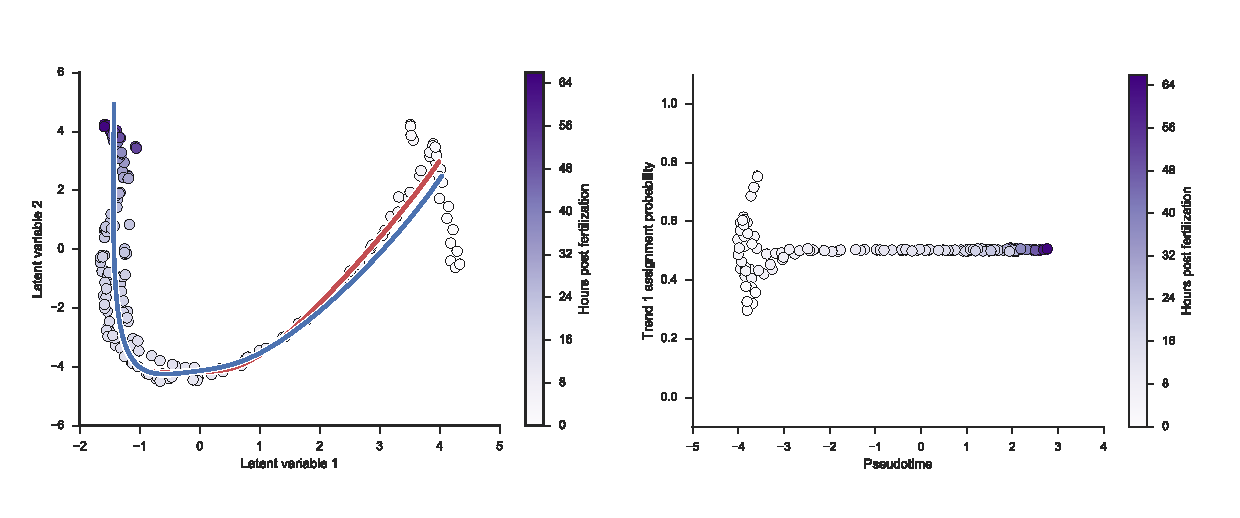
\includegraphics[width=0.95\textwidth]{frog-illustration.pdf}
    \caption{Summary of \name{GPfates} result of \citet{Owens2016-op} developing frog embryo data.}
    \label{fig:owens}
\end{figure}

No strong bifurcation is detected, and thus we skipped gene bifurcation analysis. The single-trend model explains the data well. Some heterogeneity can be seen in the early part of the time course. This might suggest that expression is somewhat noisy in extremely early embryos, but not in a way that indicates discrete cell populations.

\section{Comparison to other pseudotime and bifurcation methods} \label{sec:bif-comparison}

We compared \name{GPfates} with various methods inferring pseudotime and bifurcation events: Wishbone \cite{Setty2016-ie}, Monocle2\footnote{http://cole-trapnell-lab.github.io/monocle-release/articles/v2.0.0/}, Diffusion Pseudotime \cite{Haghverdi2016-tm}, SCUBA \cite{Marco2014-rf} and Mpath \cite{Chen2016-ar}. We applied the methods to our data and different public developmental data sets mentioned earlier. Note that the developmental embryonic frog data was treated as a negative control to investigate if methods are able to detect false positives, i.e. identifying branches when they do not exist.

\begin{figure}
    \centering
    \includegraphics[width=0.8\textwidth]{"results_malaria"}
    \caption[Output of bifurcation methods applied to malaria data]{\textbf{Output of bifurcation methods applied to malaria data.} (A) Wishbone results showing the branching structure colored by time points (left) and inferred branches (right). (B) Minimum spanning tree on cells generated by Monocle2. Cells are colored by time points (left) and inferred cell states (right). (C) Visualisation of diffusion maps in DPT colored by time points (left) and inferred branches (right). (D) Lineage tree by SCUBA reports no bifurcation. Sizes of bubbles are according to number of cells. (E) MPath's minimum spanning tree: First number corresponds to the collection time, second number corresponds to the landmark cluster. (F) \name{GPfates} trajectory, colored by time points.}
    \label{fig:res_malaria}
\end{figure}

\begin{figure}
    \centering
    \includegraphics[width=0.8\textwidth]{"results_lung"}
    \caption[Output of bifurcation methods applied to lung data]{\textbf{Output of bifurcation methods applied to lung data.} AT2 and E18.5 cells are expected to occur in one branch. (A) Wishbone's branching structure. Cells are colored by time points (left) and inferred branches (right). (B) Minimum spanning tree generated by Monocle2. Cells are colored by time points (left) and inferred cell states (right). (C) Visualization of diffusion maps in DPT colored by time points (left) and inferred branches (right). (D) Lineage tree by SCUBA: Sizes of bubbles are according to number of cells. (E) MPath's minimum spanning tree: First number corresponds to the collection time, second number corresponds to the landmark cluster. (F) \name{GPfates} trajectory, colored by time points.}
    \label{fig:res_lung}
\end{figure}

\begin{figure}
    \centering
    \includegraphics[width=0.8\textwidth]{"results_pgc"}
    \caption[Output of bifurcation methods applied to primordial germ cell data]{\textbf{Output of bifurcation methods applied to primordial germ cell data.} Bifurcation event is expected to split female and male cells. (A) Wishbone results colored by time points (left), sex (middle) and inferred branches (right). (B) Monocle2 results colored by time points (left), sex (middle) and inferred cell states (right). (C) DPT results colored by time points (left), sex (middle) and inferred branches (right). (D) SCUBA result: Sizes of bubbles are according to number of cells. (E) MPath result: First number corresponds to the collection time, second number corresponds to the landmark cluster. (F) \name{GPfates} trajectory, colored by time points. Squares corresponds to male, triangles to female cells.}
    \label{fig:res_pgc}
\end{figure}

\begin{figure}
    \centering
    \includegraphics[width=0.8\textwidth]{"results_frog"}
    \caption[Output of bifurcation methods applied to developing frog data]{\textbf{Output of bifurcation methods applied to developing frog data.} Treated as a negative control, no branching events should be reported. Please note, Mpath failed to model on developmental frog data. (A) Wishbone results colored by time points (left) and inferred branches (right). (B) Monocle2 results colored by time points (left) and inferred cell states (right). (C) DPT results colored by time points (left) and inferred branches (right). (D) SCUBA result: Sizes of bubbles are according to number of cells. (E) \name{GPfates} trajectory, colored by time points.}
    \label{fig:res_frog}
\end{figure}

The results are summarized in Fig. \ref{fig:res_malaria} through \ref{fig:res_frog}. In order to validate the approaches, we counted the number of bifurcation events for each method in each data set and compared it to the expected number of bifurcations (Table \ref{tab:alternatives_out}).

\begin{figure}
    \centering
    \includegraphics[width=\textwidth]{"realtime_vs_pseudotime_accuracy"}
    \caption[Accuracy of bifurcation methods]{\textbf{Accuracy of bifurcation methods.} Spearman's rank correlation was calculated by comparing the real time and the inferred pseudotime.}
    \label{fig:real_vs_pseudo}
\end{figure}

Furthermore, we assessed the accuracy of a method by calculating Spearman's rank correlation between the inferred pseudotime and the real time in a given data set (Figure \ref{fig:real_vs_pseudo}). For this analysis only Wishbone, Monocle2 and DPT could be considered as the SCUBA and Mpath tools do not report an inferred pseudotime which can be parsed.

Monocle2 and GPLVM perform similarly with a high accuracy ($>$ abs(0.80) Spearman's correlation) on public data. However, Monocle2 as well as Wishbone and DPT failed to assign the correct temporal order with regard to the malaria infection data. Overall, applying Wishbone and DPT to the data sets they achieved poor to moderate accuracy, except for Wishbone performing well on the frog data, and DPT performing well on developmental lung data.

Concerning the bifurcation event in developing lung data, most of the methods cluster AT2 and E18.5  cells into one branch which has been confirmed in a previous study \cite{Treutlein2014-rz}. However, in primordial germ cell data none of the published methods were able to detect branching  events between male and female cells. With regard to the frog embryonic development study only SCUBA reflects the non-branching structure of the data. All other public methods report a branching point.

\section{Discussion}

We have demonstrated the applicability of our \name{GPfates} method, where we use latent variable modeling to infer temporal expression dynamics, and Gaussian process mixture modeling for identifying diverging global trends. The method has been investigated in terms of robustness, and applied on several simulated and real data sets showing good results.

Of course there is no silver bullet for these sorts of problems, and it would not be surprising if other methods than the ones we have used work better for some biological systems. Nevertheless, we have illustrated that the main component, the Gaussian process mixture modeling, is compatible with other methods in these cases.

A benefit from the methods we use is that diagnostics such as marginal likelihood can be used to aid the user with regards to the models to use. Still, the user will need to keep the biological system in mind, and be critical of results.

\begin{sidewaystable}
\centering
\begin{tabularx}{0.8\textwidth}{lll}
\textbf{Pseudotime Method} & \textbf{Strategy} & \textbf{OMGP Compatibility} \\
\hline \\ 
Wishbone & Diffusion maps on reduced k-NN & Yes \\
\cite{Setty2016-ie} & graph (using waypoints) & \\ & & \\
Monocle2 Pseudotime &  Minimum Spanning Tree path length & Yes \\
\cite{Trapnell2014-cn} & in 2D DDRTree space &  \\ & &  \\
Diffusion maps & Spectral embedding of data manifold & With postprocessing, e.g. DPT \\
\cite{Haghverdi2015-ig} & & \cite{Haghverdi2016-tm} \\ & & \\
Wanderlust & Heuristic k-NN graph geodesic distance & Yes \\
\cite{Bendall2014-kg} & & \\ & & \\
GPLVM & Latent data parametrization & Yes  \\ & & \\
\end{tabularx}
\begin{tabularx}{0.95\textwidth}{lllll}
 &  & \textbf{Dim. } & \textbf{Clus-} & \textbf{Diff. Expr.} \\
\textbf{Bifurcation Method} & \textbf{Strategy} & \textbf{Reduction} & \textbf{tering} & \textbf{Analysis} \\
\hline \\
Wishbone & Disagreements between shortest paths & Yes & No & No \\
\cite{Bendall2014-kg} & & & & \\ & & & &\\
Monocle2 states & Create k PQ trees from a Minimum & Yes & No & Yes \\
\cite{Trapnell2014-cn} & Spanning Tree & & & \\ & & & &\\
DPT & Switch in correlation behavior & No & No & No \\
\cite{Haghverdi2016-tm}) & & & & \\  & & & & \\
SCUBA & Transitions between clusters in pseudo-& Yes & Yes & No \\
\cite{Marco2014-rf} & time bins & & & \\  & & & & \\
Mpath & Finding Minimum Spanning Tree in & Yes & Yes & Yes \\
\cite{Chen2016-ar} & neighborhood graph of landmarks &  & &  \\ & & & & \\
OMGP & Model data as mixture of continuous& Yes & No & No \\
& processes & & & \\
\end{tabularx}
\caption{Examples of common pseudotime- and bifurcation methods.}
\label{tab:alternatives}
\end{sidewaystable}

\begin{sidewaystable}
\centering
\begin{tabularx}{0.95\textwidth}{lllll}
 & \textbf{Malaria} & \textbf{Lung} & \textbf{PGC} & \textbf{Frog} \\
 & This work & \cite{Treutlein2014-rz} & \cite{Guo2015-ao} & \cite{Owens2016-op} \\
\hline \\ 
Wishbone & 1 (1) & 1 (1) & 1 (1) & 1 (0) \\
Monocle2 & 7 (1) & 1 (1) & 2 (1) & 1 (0) \\
DPT & 1 (1) & 0 (1) & 1 (1) & 1 (0) \\
SCUBA & 0 (1) & 0 (1) & 0 (1) & 0 (0) \\
Mpath & 1 (1) & 2 (1) & 1 (1) & NA (0) \\
\end{tabularx}
\caption{Number of detected (and expected) bifurcations of other methods.}
\label{tab:alternatives_out}
\end{sidewaystable}
